We now sketch the representations underpinning our approach. We define several models: an object model (partial and acquired from sensing); a model of the contact between a finger link and the object; a model of the whole hand configuration; and a model of the reach to grasp trajectory. First we describe the kernel density representation for all these models. Then we describe the surface features we use to encode some of these models. Then we follow with a description of each model type. Throughout we assume that the robot's hand comprises $N_L$ rigid \emph{links}: a palm, and several phalanges or links. We denote the set of links $L =\{L_i\}$. 

\subsection{Kernel Density Estimation}
\label{sec:kde}
$SO(3)$ denotes the group of rotations in three dimensions. A feature belongs to the space $SE(3) \times \mathbb R^2$, where $SE(3) = \mathbb R^3 \times SO(3)$ is the group of 3D \emph{poses}, and surface descriptors are composed of two real numbers. We extensively use probability density functions (PDFs) defined on $SE(3) \times \mathbb R^2$.  We represent these PDFs non-parametrically with a set of $K$ features (or particles) $x_j$
\begin{equation}
S = \left\lbrace x_j : x_j \in \mathbb R^3 \times SO(3) \times \mathbb R^2 \right\rbrace_{j \in [1,K]}.
\end{equation}
The probability density in a region is determined by the local density of the particles in that region. The underlying PDF is created through \emph{kernel density estimation} \cite{silverman1986a}, by assigning a kernel function $\mathcal{K}$ to each particle supporting the density, as
\begin{equation}\label{eq:d}
\pdf(x) \simeq \sum_{j=1}^K w_j \mathcal{K}(x| x_{j}, \sigma),
\end{equation}
where  $\sigma \in \mathbb R^3$ is the kernel bandwidth and $w_j \in \mathbb R^{+}$ is a weight associated to $x_j$ such that $\sum_j w_j = 1$. We use a kernel that factorises into three functions defined by the separation of $x$ into $p \in \mathbb R^3$ for position, a quaternion $q \in SO(3)$ for orientation, and $r \in \mathbb R^2$ for the surface descriptor. Furthermore, let us denote by $\mu$ another feature, and its separation into position, orientation and a surface descriptor. Finally, we denote by $\sigma$ a triplet of real numbers:
\begin{subequations}
\begin{align}
x &= (p, q, r),\\
\mu &= (\mu_p, \mu_q, \mu_r),\\
\sigma &= (\sigma_p, \sigma_q, \sigma_r).
\end{align}
\label{eq:feature}
\end{subequations}
We define our kernel as
\begin{equation}\label{eq:kernel_in_se3}
\mathcal{K}(x| \mu, \sigma) = \mathcal{N}_3(p| \mu_p, \sigma_p) \Theta(q| \mu_q, \sigma_q) \mathcal{N}_2(r| \mu_r, \sigma_r)
\end{equation}
where $\mu$ is the kernel mean point, $\sigma$ is the kernel bandwidth, $\mathcal{N}_n$ is an $n$-variate isotropic Gaussian kernel, and ${\Theta}$ corresponds to a pair of antipodal von Mises-Fisher distributions which form a Gaussian-like distribution on $SO(3)$ \cite{fisher1953a,sudderth2006a}. The value of ${\Theta}$ is given by
\begin{equation}
\Theta(q|\mu_q, \sigma_q) = C_4(\sigma_q) \frac {e^{\sigma_q \; \mu_q^T q} + e^{-\sigma_q \; \mu_q^T q}}2
\end{equation}
where $C_4(\sigma_q)$ is a normalising constant, and $\mu_q^T q$ denotes the quaternion dot product.

Using this representation, conditional and marginal probabilities can easily be computed from \eq\eqref{eq:d}. The marginal density $\pdf(r)$ is computed as
\begin{multline}\label{eq:marginal}
\pdf(r)\\
= \iint \sum_{j=1}^K w_j \mathcal{N}_3(p| p_i, \sigma_p) \Theta(q| q_i, \sigma_q) \mathcal{N}_2(r| r_i, \sigma_r) \textnormal{d}p\textnormal{d}q \\
=  \sum_{j=1}^K w_j \mathcal{N}_2(r| r_j, \sigma_r),
\end{multline}
where $x_j = (p_j, q_j, r_j)$.
The  conditional density $\pdf(p,q|r)$ is given by
\begin{multline}\label{eq:conditional}
\pdf(p,q|{r}) = \frac{\pdf(p, q, {r})}{\pdf({r})}\\
= \frac{\sum_{j=1}^K w_j \mathcal{N}_2({r}| r_j, \sigma_r) \mathcal{N}_3(p| p_j, \sigma_p) \Theta(q|q_j, \sigma_q)}{\sum_{j=1}^K w_j \mathcal{N}_2({r}| r_j, \sigma_r)}. 
\end{multline}

\subsection{Surface Features}
\label{sec:surface_features}

All objects considered in the paper are represented by point clouds for the purpose of learning and testing. Test object models were constructed from a single view with a depth camera, and were thus incomplete5. We directly augment these points with a frame of reference and a surface feature that is a local curvature descriptor. For compactness, we also denote the pose of a feature as $v$. As a result,
\begin{equation}
x = (v, r), \qquad v = (p, q).
\label{eq:surface.feature}
\end{equation}

The surface normal at $p$ is computed from the nearest neighbours of $p$ using a PCA-based method (e.g. \cite{kanatani2005statistical}). The surface descriptors are the local \emph{principal curvatures} \cite{spivak1979comprehensive}. Their directions are denoted $k_1, k_2 \in \mathbb R^3$, and the curvatures along $k_1$ and $k_2$ form a $2$-dimensional feature vector $r = (r_1, r_2) \in \mathbb R^2$. %The surface normals and curvatures are computed using the PCL library \citep{Rusu_ICRA2011_PCL}.
The surface normal and the principal directions define the orientation $q$ of a frame that is associated with the point $p$. 

\subsection{Object Model}
\label{sec:object_model}

Thus, given a point cloud of object $n = 1..N_O$, a set of $K_{O_n}$ features $\lbrace (v_{jn}, r_{jn}) \rbrace$ can be computed. This set of features defines, in turn, a joint probability distribution, which we call the \emph{object model}:
\begin{equation}
\om_n(v, r) \equiv \pdf^\om(v, r) \simeq \sum_{j=1}^{K_{O_n}} w_{jn} \mathcal{K}(v, r|{x_{jn}}, \sigma_{x})
%RD: mu and sigma are not properly defined.
\label{eq:om}
\end{equation}
where $\om$ is short for $\pdf^\om$, $x_{jn} = (v_{jn}, r_{jn})$,  $\mathcal{K}$ is defined in \eq\eqref{eq:kernel_in_se3} with bandwidth $\sigma_{x} = (\sigma_{v}, \sigma_{r})$, and where all weights are equal, $w_{jn} = 1/{K_{O_n}}$. In summary this object model $\om$ represents the object as a pdf over surface normals and curvatures.

\section{LEARNED MODELS}

We now describe the representations for each of the three models that are learned from a set of grasp examples. We start with the contact receptive field, proceed with the contact model, the equilibrium state hand configuration model, and finish with the reach to grasp model.

\subsection{Contact Receptive Field}\label{sec:contact_recfield}

\begin{figure}[t]
\centerline{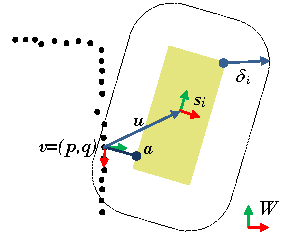
\includegraphics[width=6cm]{resources/contact}}
\caption[Contact receptive field]{The contact receptive field $\rf$ associated with the $i$-th link $\rl_i$ (solid yellow block) with link pose $s_i$. The black dots are samples from the surface of an object. The distance $a$ between feature $v$ and the closest point $a$ on the link's surface is shown. The rounded rectangle illustrates the cut-off distance $\delta_i$. The poses $v$ and $s_i$ are expressed in the world frame $W$. The arrow $u$ is the pose of $\rl_i$ relative to the frame for the surface feature $v$.}
\label{fig:contact_recfield}
\end{figure}

The \textit{contact receptive field} $\rf_i$ is a region of space relative to the associated robot link $\rl_i$ (see \fig\ref{fig:contact_recfield}) which specifies the neighbourhood of a particular robot link. The contact receptive field $\rf_i$ is realised as a function of surface feature pose $v$:
\begin{equation}
\rf_{i} : SE(3) \rightarrow [0, 1]
\label{eq:contact_recfield_model}
\end{equation}
the value of which determines the relevance of a particular surface feature $x = (v, r)$ to a given link $\rl_i$ in terms of the likelihood of the physical contact. We use contact receptive fields which are family of parameterised functions for which the value falls off quickly with the distance to the link:
\begin{equation}
\rf_{i}(v|\lambda_i,\delta_i) = \begin{cases}\exp(-\lambda_i ||p-a||^2) \quad &\textnormal{ if } ||p-a|| < \delta_i\\
0 \quad &\textnormal{ otherwise},\end{cases}
\label{eq:contact_recfield_func}
\end{equation}
where $\lambda_i \in \mathbb R^{+}$ and $a$ is the point on the surface of $\rl_i$ that is closest to $v = (p, q)$. This means that the contact contact receptive field will only take account of the local shape, while falling off smoothly. A variety of monotonic, fast declining functions could be used instead.


\subsection{Contact Model}\label{sec:contact.model}

Let us assume that we have as many grasp examples of the same grasp type $g$ as the number of objects $N_O$. We denote by $u_{ij} = (p_{ij}, q_{ij})$ the pose of $\rl_i$ relative to the pose $v_j$ of the $j$-th object feature. In other words, $u_{ij}$ is defined as
\begin{equation}
u_{ij} = v_j^{-1} \circ s_i,
\label{eq:local.pose}
\end{equation}
where $s_i$ denotes the pose of $\rl_i$, $\circ$ denotes the pose composition operator, and $v_j^{-1}$ is the inverse of $v_j$, with $v_j^{-1} = (-q_j^{-1}p_j, q_j^{-1})$ (see \fig\ref{fig:contact_recfield}). 

Contact model $\cm_{in}$ encodes the joint probability distribution of surface features of object $n$ and of the 3D pose of the $i$-th hand link in the equilibrium state. Let us consider the hand as having grasped given training object $n$. The contact model for link $\rl_i$ is denoted by
\begin{equation}\label{eq:M}
\cm_{in}(U, R) \equiv \pdf^\cm_{in}(U, R)
\end{equation}
where $\cm_i$ is short for $\pdf^\cm_{in}$, $R$ is the random variable modelling surface features of object $n$, and $U$ models the pose of $\rl_i$ \emph{relative} to the frame of reference defined by the directions of principal curvature and the surface normal. In other words, denoting realisations of $R$ and $U$ by $r$ and $u$, $\cm_{in}(u, r)$ is proportional to the probability of finding $\rl_i$ at pose $u$ relative to the frame of a nearby object surface patch that exhibits features (principal curvatures) equal to $r$.

The contact model of object $n$ is estimated as
\begin{equation}\label{eq:cm_n}
\begin{split}
&\cm_{in}(u, r) \simeq \frac 1Z \int \mathcal{K}(u|v^{-1}s_i, \sigma_\cm) \om_{n}(v, r) \rf_{i}(v) dv\\
&= \frac 1Z \sum_{j=1}^{K_{O_n}} w_{jn} \mathcal{K}(u|v_{jn}^{-1}s_i, \sigma_v) \mathcal{N}_2({r}| r_{jn}, \sigma_r) \rf_{i}(v_{jn})
\end{split}
\end{equation}
where $Z \in \mathbb R^+$ is a normalising constant and $\mathcal{K}$ is kernel function \eqref{eq:kernel_in_se3} defined at poses from \eq\eqref{eq:local.pose}, and where we have performed integration over all kernels of the object model \eqref{eq:om} which uniquely determine poses $v$.

We also introduce \textit{contact model norm}, which estimates the likelihood of a physical contact of link $i$ with surface features of object $n$:
\begin{equation}\label{eq:cm_norm}
\|\cm_{in}\| = \frac 1Z \sum_{j=1}^{K_{O_n}} w_{jn} \rf_{i}(v_{jn})
\end{equation}
where $Z \in \mathbb R^+$ is a normalising constant.

\subsection{Contact Model Selection}

The overall number of non-empty contact models $\cm_{in}$ for the example grasp $n$ is usually smaller than the number of links $N_L$ of the robot hand. The contact selection procedure determines which contact models should be instantiated for a given grasp type. The procedure starts with comparing contact model norms \eqref{eq:cm_norm} to the average model norm for all grasp examples and all robot links. The results of this comparison are stored in binary variables $b_{in}$:
\begin{equation}
b_{in} = \begin{cases} 1 \quad &\textnormal{ if } \frac{N_L N_O \|\cm_{in}\|}{\sum_{jk}\|\cm_{jk}\|} > \eta_i \\
0 \quad &\textnormal{ otherwise},\end{cases}
\label{eq:cm_n_binary}
\end{equation}
where $\eta_i \in \mathbb{R}^+$ is a threshold constant, $N_L$ is the number of hand links and $N_O$ is the number of training objects.

The contact model $\cm_i$ is instantiated if the total number of non-empty contact models, determined by $b_{in}$, is higher than some minimum value given the total number of objects or training grasps $N_O$. This is encoded in binary variable $c_i$:
\begin{equation}
c_i = \begin{cases} 1 \quad &\textnormal{ if } \frac{1}{N_O} \sum_k b_{ik} > \zeta\\
0 \quad &\textnormal{ otherwise},\end{cases}
\label{eq:cm_binary}
\end{equation}
where $\zeta \in \mathbb{R}^+$ is a threshold constant. The contact model $\cm_i$ is then constructed as a mixture of $\cm_{in}$ as follows:
\begin{equation}\label{eq:cm}
\cm_{i}(u, r) = \sum_{n=1}^{N_O} c_{i} b_{in} \cm_{in}(u, r)
\end{equation}

We denote the set of contact models learned for a particular grasp type $g$ as $\mathcal{\cm}^g=\{\mathcal{\cm}^g_i\}$. The parameters $\lambda$, $\eta$, $\zeta$ and $\sigma_{p}$, $\sigma_{q}$, $\sigma_{r}$ were chosen empirically. The time complexity for learning each contact model $\cm_{in}(u, r)$ from an example grasp is $\Omega(T_i K_{O_n})$ where $T_i$ is the number of triangles in the tri-mesh describing hand link $i$, and $K_{O_n}$ is the number of points of object $n$.


%\begin{figure}[t]
%\centerline{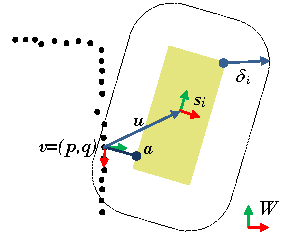
\includegraphics[width=5cm]{resources/contact}}
%\caption[Contact model]{Contact model. The figure shows the $i$-th link $\rl_i$ (solid block) and its pose $s_i$. The black dots are samples of the surface of an object. The distance $a_{ij}$ between a feature $v_j$ and the closest point on the link's surface is shown. The rounded rectangle illustrates the cut-off distance $\delta_i$. The poses $v_j$ and $s_i$ are expressed in the world frame $W$. The arrow $u_{ij}$ is the pose of $\rl_i$ relative to the frame for the surface feature $v_j$.}
%\label{fig:representations.model}
%\end{figure}
%
%A contact model $\cm_i$ encodes the joint probability distribution of surface curvatures and of the 3D pose of the $i$-th hand link in the equilibrium state. Let us consider the hand as having grasped some given training object. The contact model for link $\rl_i$ is denoted by
%\begin{equation}\label{eq:M}
%\cm_i(U, R) \equiv \pdf^\cm_i(U, R)
%\end{equation}
%where $\cm_i$ is short for $\pdf^\cm_i$, $R$ is the random variable modelling surface curvature, and $U$ models the pose of $\rl_i$ \emph{relative} to the frame of reference defined by the directions of principal curvature and the surface normal. In other words, denoting realisations of $R$ and $U$ by $r$ and $u$, $\cm_i(u, r)$ is proportional to the probability of finding $\rl_i$ at pose $u$ relative to the frame of a nearby object surface patch that exhibits principal curvatures equal to $r$.
%
%Given a set of features $\lbrace x_j \rbrace_{j=1}^{K_O}$, with $x_j = (v_j, r_j)$ and $v_j = (p_j, q_j)$, a contact model $\cm_i$ is constructed from them.  Features close to the link surface are more important than those lying far from the surface. Features are thus weighted, to make their influence on $\cm_i$  decrease with their distance to the $i^\textnormal{th}$ link. %(\fig\ref{fig:representations.modeldist.cont}). 
%We use a weighting function whose value decreases exponentially with the square distance to the link:
%\begin{equation}
%w_{ij} = \begin{cases}\exp(-\lambda ||p_j-a_{ij}||^2) \quad &\textnormal{ if } ||p_j-a_{ij}|| < \delta_i\\
%0 \quad &\textnormal{ otherwise},\end{cases}
%\label{eq:learning.modeldist.wgh}
%\end{equation}
%where $\lambda \in \mathbb R^{+}$, there is a cut-off distance $\delta_i$, and $a_{ij}$ is the point on the surface of $\rl_i$ that is closest to $p_j$. The intuitive motivation for this choice is that we require a weight function that falls off quickly so that the contact model will only take account of the local shape, while falling off smoothly.
%
%Let us denote by $u_{ij} = (p_{ij}, q_{ij})$ the pose of $\rl_i$ relative to the pose $v_j$ of the $j^{\mathnormal{th}}$ surface feature. In other words, $u_{ij}$ is defined as
%\begin{equation}
%u_{ij} = v_j^{-1} \circ s_i,
%\label{eq:local.pose}
%\end{equation}
%where $s_i$ denotes the pose of $\rl_i$, $\circ$ denotes the pose composition operator, and $v_j^{-1}$ is the inverse of $v_j$, with $v_j^{-1} = (-q_j^{-1}p_j, q_j^{-1})$ (see \fig\ref{fig:representations.model}). The contact model is estimated as
%\begin{equation}
%\cm_i(u,r) \simeq \frac 1Z \sum^{K_{M_i}}_{j=1} w_{ij}\mathcal{N}_3(p|{p_{ij}}, \sigma_{p}) \Theta(q|{q_{ij}}, \sigma_{q}) \mathcal{N}_2(r|{r_j}, \sigma_{r})
%\label{eq:cm}
%\end{equation}
%where $Z$ is a normalising constant, $u = (p, q)$, and where $K_{M_i} \leq K_O$ is a number of features which are within cut-off distance $\delta_i$ to the surface of link $\rl_i$. If the number of features $K_{M_i}$ of contact model $\cm_i$ is not sufficiently large, contact model $\cm_i$ is not instantiated and is excluded from any further computation. Consequently, the overall number of contact models $N_M$ is usually smaller than the number of links $N_L$ of the robotic hand. We denote the set of contact models learned from a grasp example $g$ as $\mathcal{M}^g=\{\mathcal{M}^g_i\}$. 
%%Sum~\eqref{eq:cm} involves only terms for which $x_j = ((p_j, q_j), r_j)$ belong to the neighbourhood of $\rf_i$, $\lbrace x_j: ||p_j-a_{ij}|| \leq \delta, \delta \in \mathbb R^{+} \rbrace$. If the neighbourhood of a particular link $i$ is empty, i.e. $K_{M_i} = 0$, the corresponding contact model is not instantiated and it is excluded from any further computation.
%The parameters $\lambda$ and $\sigma_{p}$, $\sigma_{q}$, $\sigma_{r}$ were chosen empirically. The time complexity for learning each contact model from an example grasp is $\Omega(T K_O)$ where $T$ is the number of triangles in the tri-mesh describing the hand links, and $K_O$ is the number of points in the object model.

%\begin{figure}[t]
%\centering{
%\subfloat[]{\includegraphics[height=3.4cm]{resources/example1}}\quad
%\subfloat[]{\includegraphics[height=3.4cm]{resources/example2}}\quad
%\subfloat[]{\includegraphics[height=3.4cm]{resources/example5}}
%}
%\caption[Hand-object contact]{Example top grasp of a mug represented by a point cloud (panel a). The dotted regions are rays between features and the closest hand link surfaces (panel b). The black curves with frames at the fingertips represent the range of hand configurations in \eq\eqref{eq:hc} (panel c).}
%\label{fig:representations.modeldist.cont}
%\end{figure}

\subsection{Equilibrium State Hand Configuration Model}

The equilibrium state hand configuration model, denoted $h^e_c(j) \in \mathbb R^D$, for the grasp examples $n = 1 \ldots N_O$ within the set of $n$ training examples of a particular grasp type $g$. The purpose of this model is to restrict the grasp search space (during grasp transfer) to hand configurations that resemble those observed during training. We combine the configurations for the examples $n = 1 \ldots N_O$ to create a single mixture model density:
\begin{equation}
\hc^g(h^e_c) \equiv \sum_{n=1}^{N_O} \mathcal{N}_D(h^e_c|h^e_c(n), \sigma_{h^e_c}) 
\label{eq:hc}
\end{equation}
This expresses a density over hand configurations in the equilibrium state for a grasp type $g$.

\subsection{Reach to Grasp Model}

For a particular grasp type, in addition to modelling the equilibrium states of the hand, we must also model the trajectories taken to reach those equilibrium states. A single reach to grasp trajectory for an underactuated hand has three elements: the tool centre point (wrist) trajectory, the hand configuration trajectory, and the motor signal trajectory. We assume that a trajectory starts at time $t_0$ and ends in the equilibrium state at time $t_e$. We denote the wrist trajectory $h_w^{0:e}$, the hand configuration trajectory $h_c^{0:e}$, and the motor signal trajectory $h_m^{0:e}$ respectively. The motor signal can be a wide variety of signals in practice. Here we choose it to be the position of the single actuator. When the hand is not in contact with an object the motor signal and the wrist pose together determine the hand configuration. When in contact, the actual hand configuration will differ. The reach to grasp model is simply the concatenation of each component $(h_w^{0:e} , h_c^{0:e} , h_m^{0:e})$. The set of reach to grasp trajectory models define an attractor basin, leading towards the final hand configuration.

In the next section we explain how we gather the grasp examples that are used to learn these models. Then in Section~\ref{sec:infer} the inference method---by which the models are used to generate grasps for new objects---is described.
